\subsection{Algorithms Chosen}
\label{sec:choice}

Choosing which algorithms to test is usually based on what is being predicted
and intuition regarding strengths and weaknesses of different optimization
methods.  

For a benchmarking excercise, some machine learning approaches here were chosen
based on previous work \cite{dayman_feasibility_2013}: nearest neighbor and
ridge regression. These are useful because they are simple, providing a
dissimilarity-based model and a linear regression-based model, respectively. If
more complex algorithms are not required to obtain useful results, then there
is no need to use more computationally expensive options. However, hedging on
the fact that more complex models will be needed, this work also employs an
algorithm that is known to handle highly dimensional data sets well: support
vector regression. These algorithms were introduced in Section \ref{sec:algs}. 

\begin{table}[!htb]
  \centering
  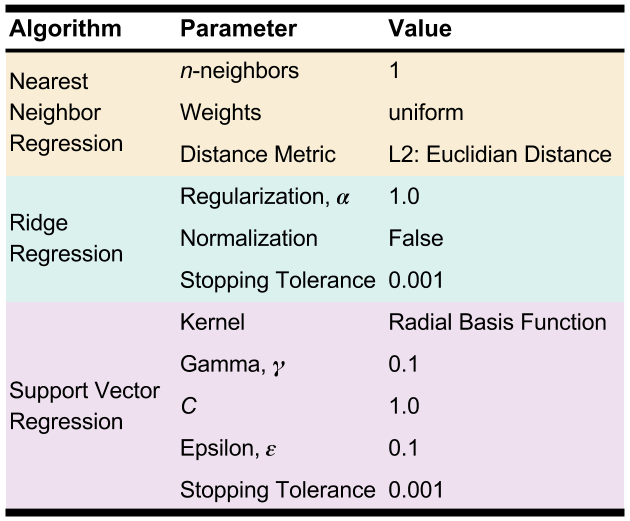
\includegraphics[width=0.8\linewidth]{./chapters/demo_method/defaults.png}
  \caption{Defaults.....................}
  \label{tbl:defaults}
\end{table}

A python-based machine learning toolkit, scikit-learn \cite{scikit}, is used to
train the models. The default parameters used for the algorithms are in
Table \ref{tbl:defaults}.

\subsection{Reactor Parameter Prediction}
\label{sec:rxtrparam}

The prediction of reactor parameters here is done with the burnup of the
\gls{SNF} to provide algorithm and corresponding model generalizability.
Following the training phase of the models, next it is important to estimate
the reactor parameter predication capabilities of those models. This is done
with a set of measurements from a test data set with samples that mimic
interdicted \gls{SNF}. The testing set has the same features as the training
set, with labels that are compared to the predicted labels. The results of each
model's prediction errors are shown in Table \ref{tbl:err}. 

\begin{table}[!htb]
  \centering
  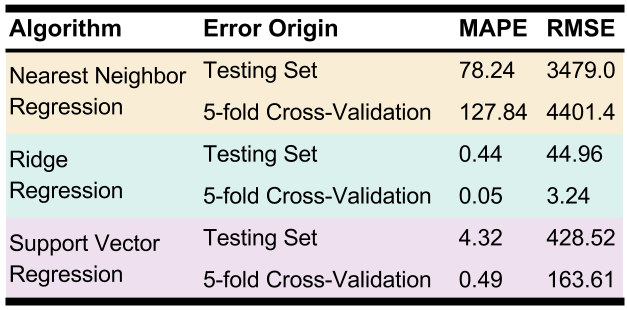
\includegraphics[width=0.8\linewidth]{./chapters/demo_method/err.png}
  \caption{Model burnup prediction errors for three algorithms}
  \label{tbl:err}
\end{table}

First shown in Table \ref{tbl:err} are testing set errors and cross-validation
errors, because although previous work uses the former, it is expected that the
latter will provide better estimates.  The models evaluated by the testing set
do not have a validation set for pre-evaluation.  The models that are evaluated
via cross-validation do not use the testing set. 

Table \ref{tbl:err} includes two error types.  For the sake of comparison to
previous work and convenient interpretation, \gls{MAPE} is tracked. However,
\gls{MAPE} requires that no true values are $0$.  The preferred method in the
community is to use \gls{RMSE} for model error estimation, so both are
tabulated.  The \gls{MAPE} shows that there are some extremely high and
extremely low errors depending on the algorithm, both of which are quite
concerning, as this indicates poor performance.  

\begin{figure}[!htb]
  \centering
  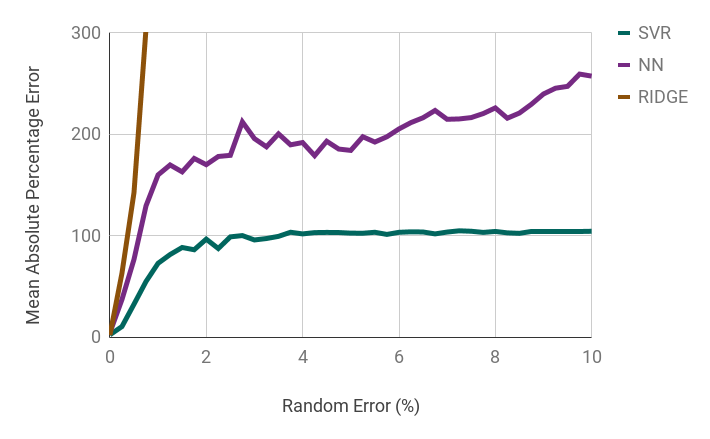
\includegraphics[width=\linewidth]{./chapters/demo_method/randerr.png}
  \caption{Results from information reduction using random error}
  \label{fig:randerr}
\end{figure}

Figure \ref{fig:randerr} shows the three algorithm's \gls{MAPE}s with respect
to the reduction of information by the introduction of random error to the
nuclide vectors as described in Section \ref{sec:inforeduc}.  \gls{SVR} is
shown to perform the best, but it quickly reaches 100\% error.  Although ridge
regression rapidly increases with any amount of error, nearest neighbor
regression shows more promise, although it reaches 257\% at 10\% error.
Overall, this performance indicates that these algorithms are unlikely to
predict burnup when faced with uncertainties in real-world measurements or
the further reduction in information from gamma detection.

Given the results in Table \ref{tbl:err} and Figure \ref{fig:randerr}, next
introduced are some diagnostic and optimization procedures that can shed light
on the performance.
